\documentclass{article}
\usepackage[utf8]{inputenc}
\usepackage{graphicx}
\usepackage{float}

\title{Testing Of Team Broadsword Access User }
\author{Bernard van Tonder }
\date{May 2017}

\begin{document}

\maketitle

\section{Service Contracts}
1.	Authenticate user\\
2.	Login\\
3.	Register\\
4.	View user profile\\
5.	Update user information\\
6.	delete user information\\
7.	Manage user information\\
    a.	Delete user\\
    b.	Add user\\
    c.	Grant admin rights\\

\subsection{Authenticate user}
\begin{figure}[ht!]
\hspace*{-2.5cm} 
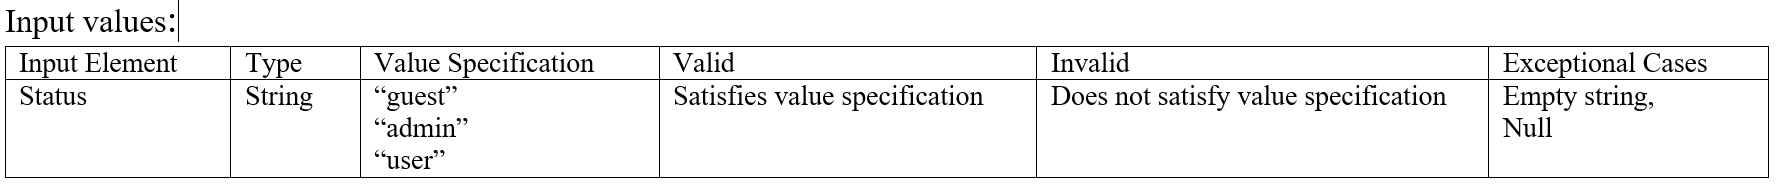
\includegraphics[width=180mm]{1.png}
\end{figure}

\begin{figure}[ht!]
\hspace*{-2.5cm} 
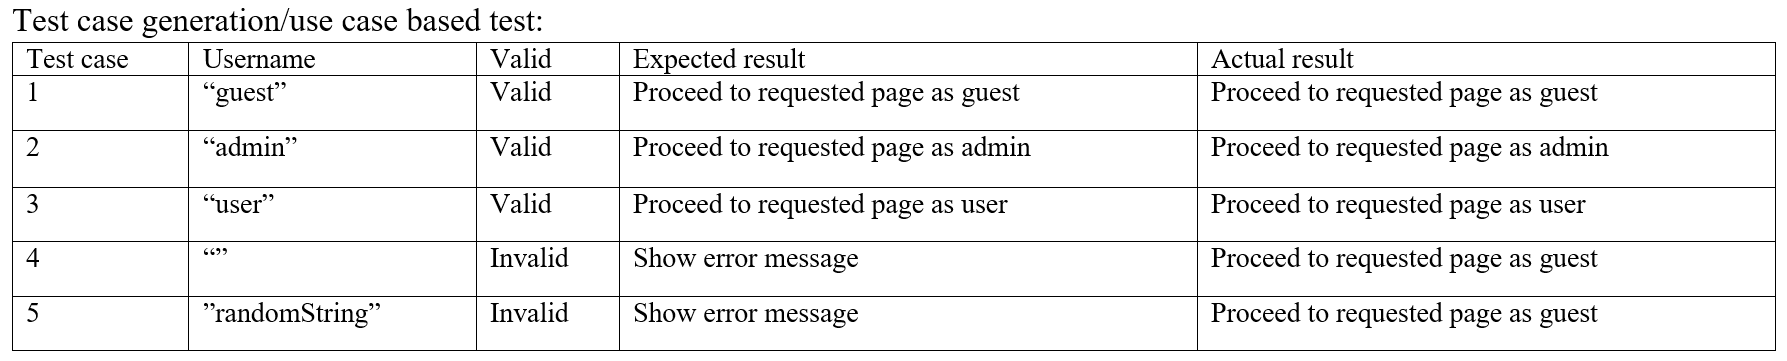
\includegraphics[width=180mm]{2.png}
\end{figure}

\subsection{Login}
\begin{figure}[ht!]
\hspace*{-2.5cm} 
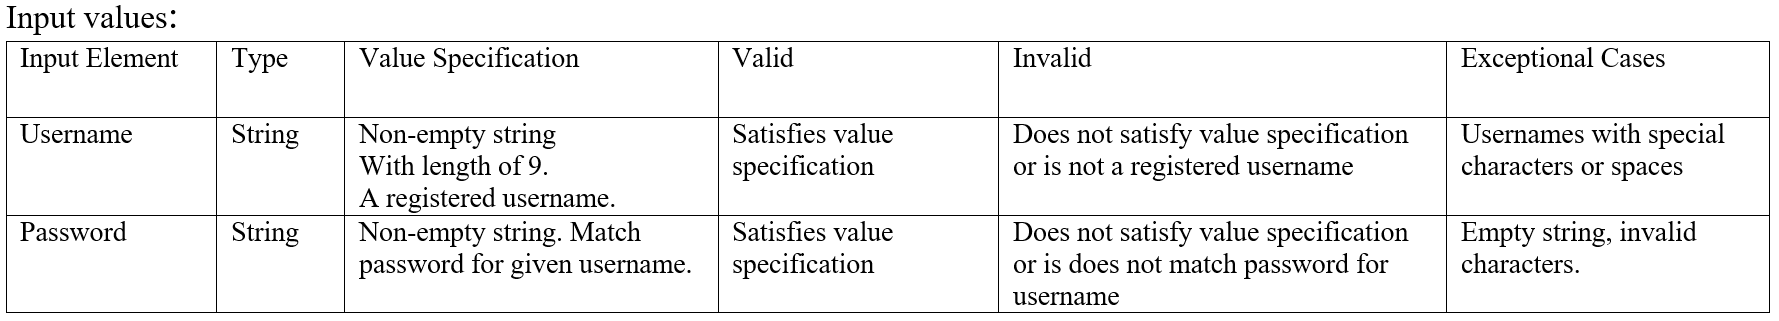
\includegraphics[width=180mm]{3.png}
\end{figure}


\begin{figure}[ht!]
\hspace*{-2.5cm} 
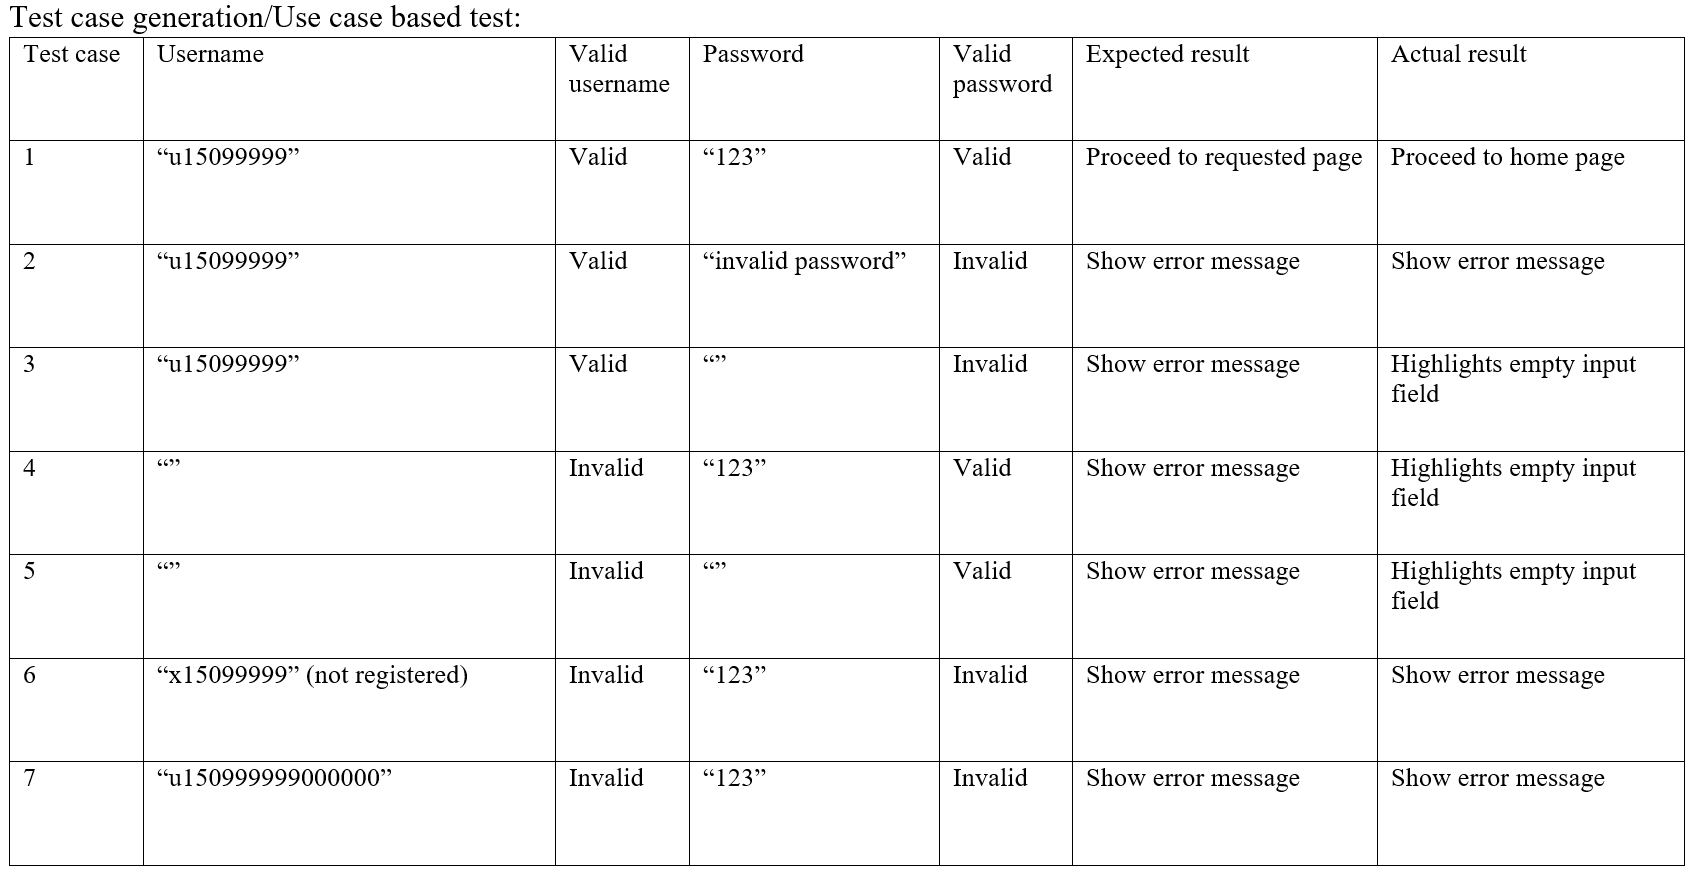
\includegraphics[width=180mm]{4.png}
\end{figure}

\subsection{Register}

\begin{figure}[H]
    \label{tab:example}
\hspace*{-2.5cm} 
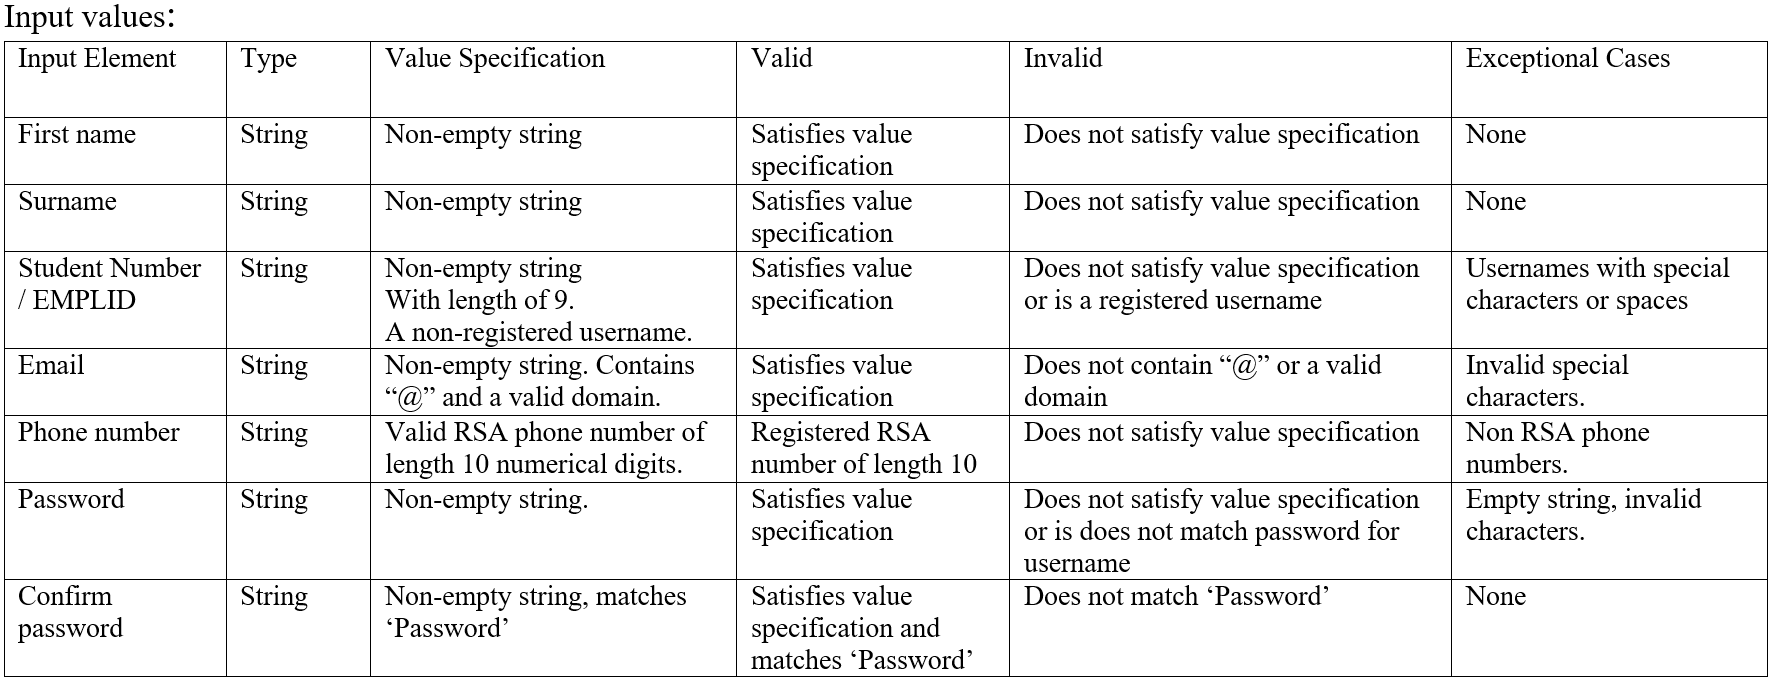
\includegraphics[width=180mm]{5.png}
\end{figure}

\begin{figure}[H]
\hspace*{-2.5cm} 
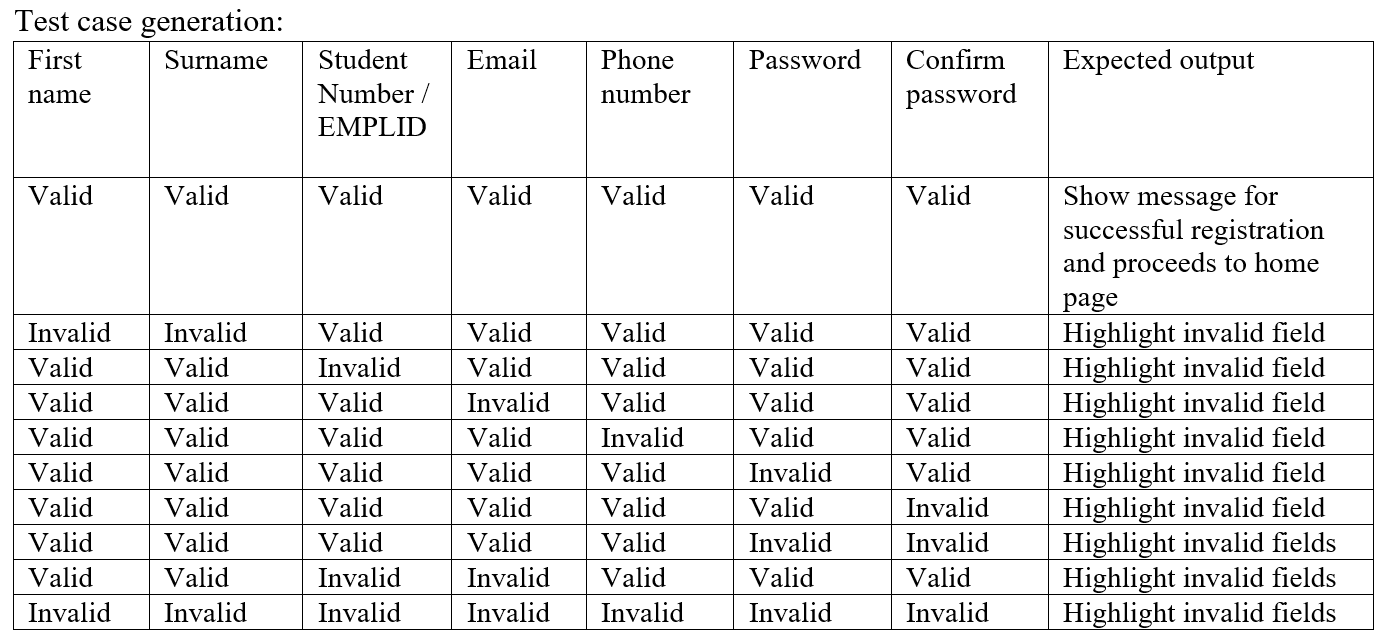
\includegraphics[width=180mm]{6.png}
\end{figure}

\begin{figure}[H]
\hspace*{-2.5cm} 
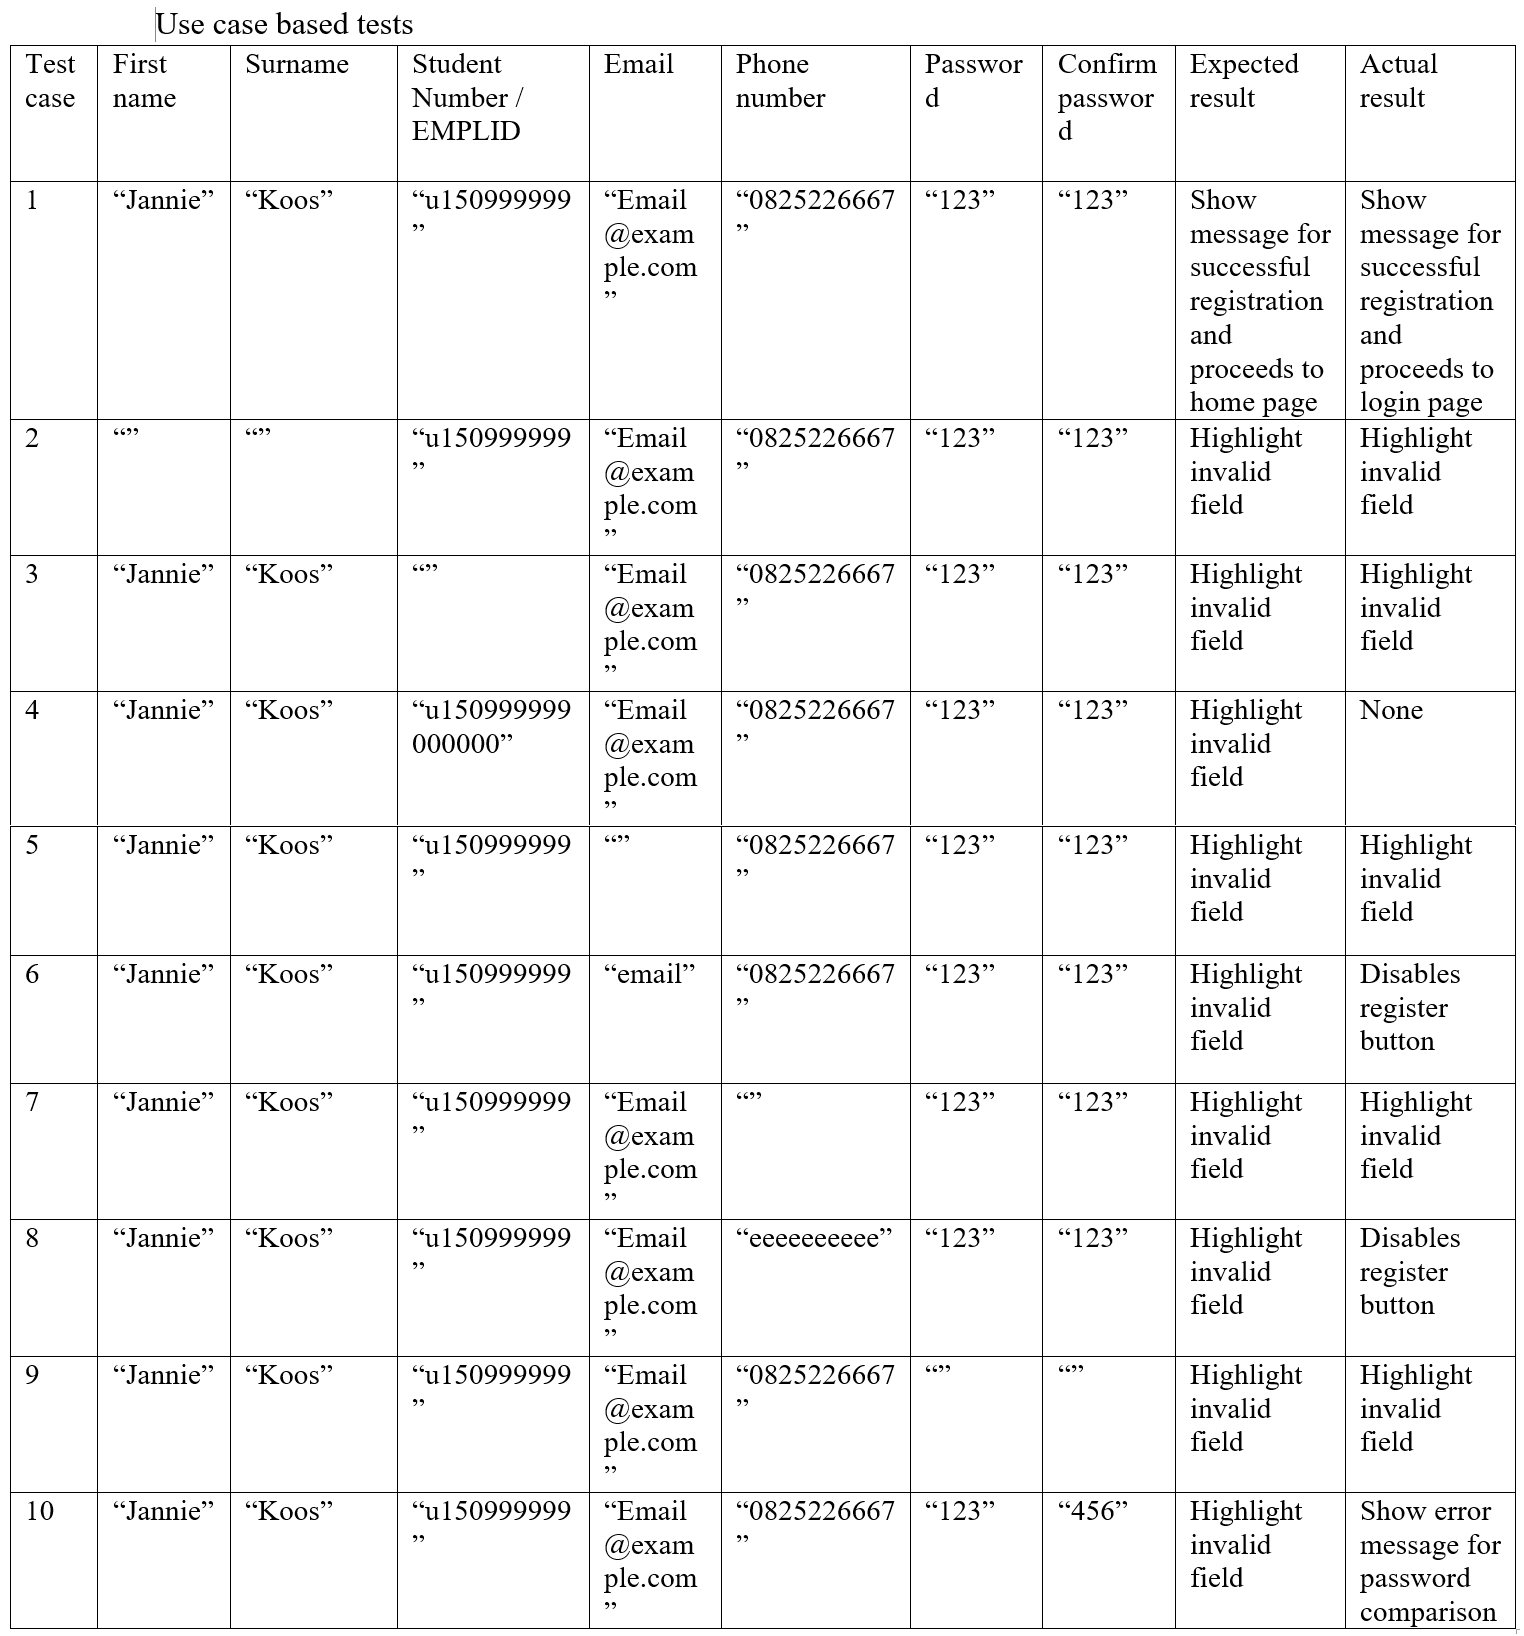
\includegraphics[width=180mm]{7.png}
\end{figure}

\subsection{View user profile}
\begin{figure}[ht!]
\hspace*{-2.5cm} 
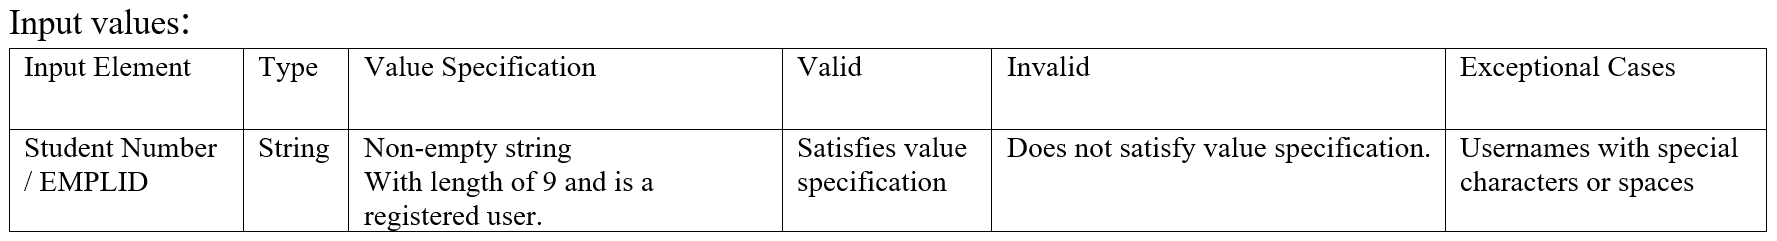
\includegraphics[width=180mm]{8.png}
\end{figure}

\begin{figure}[ht!]
\hspace*{-2.5cm} 
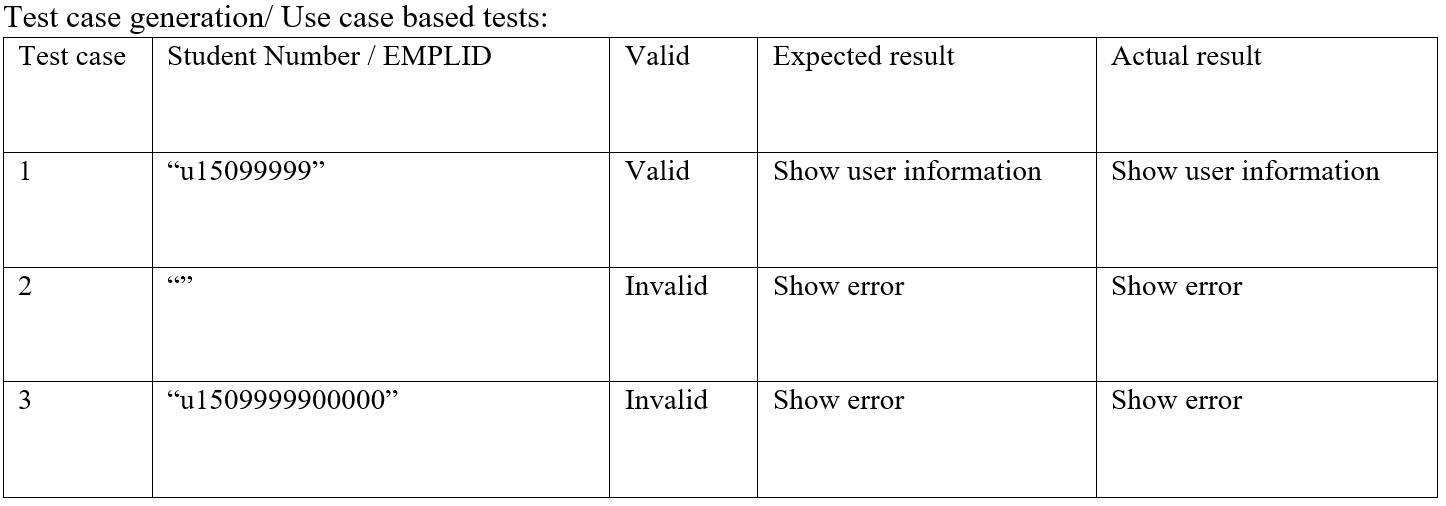
\includegraphics[width=180mm]{ViewTestCase.png}
\end{figure}

\subsection{Update user information}
\begin{figure}[H]
\hspace*{-2.5cm} 
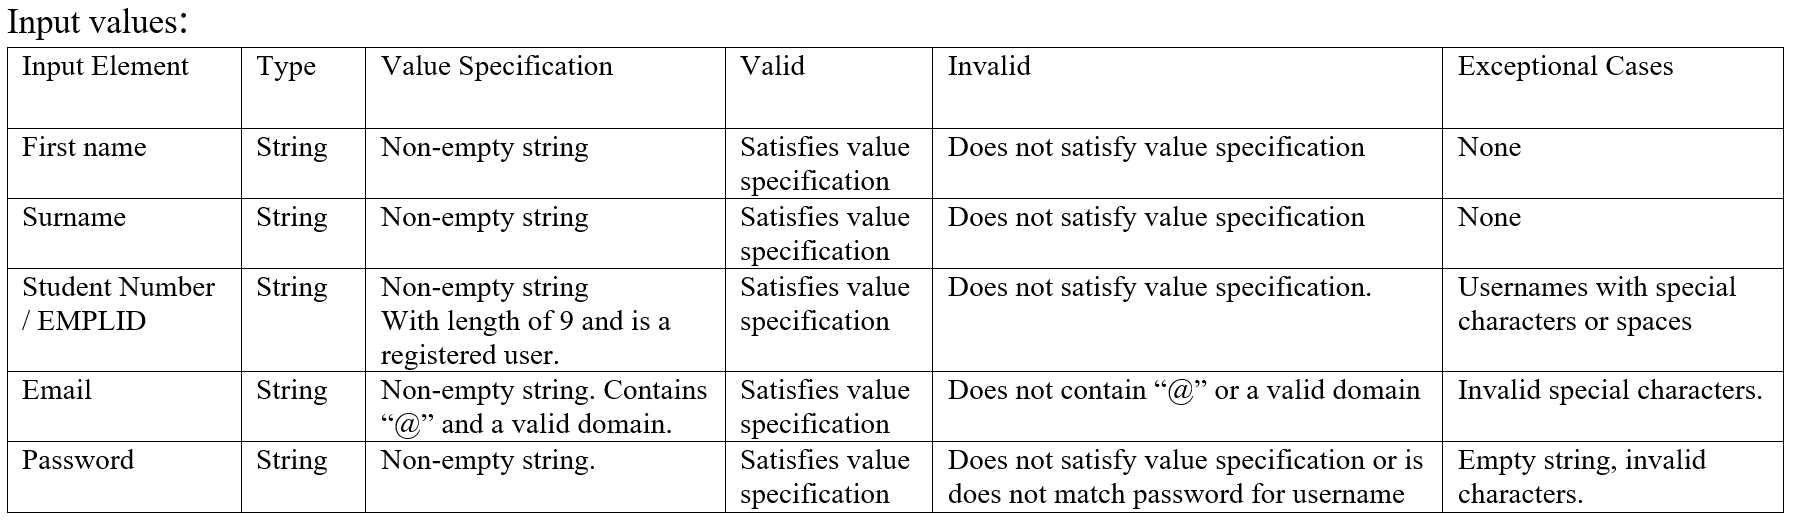
\includegraphics[width=180mm]{9.png}
\end{figure}

\begin{figure}[H]
\hspace*{-2.5cm} 
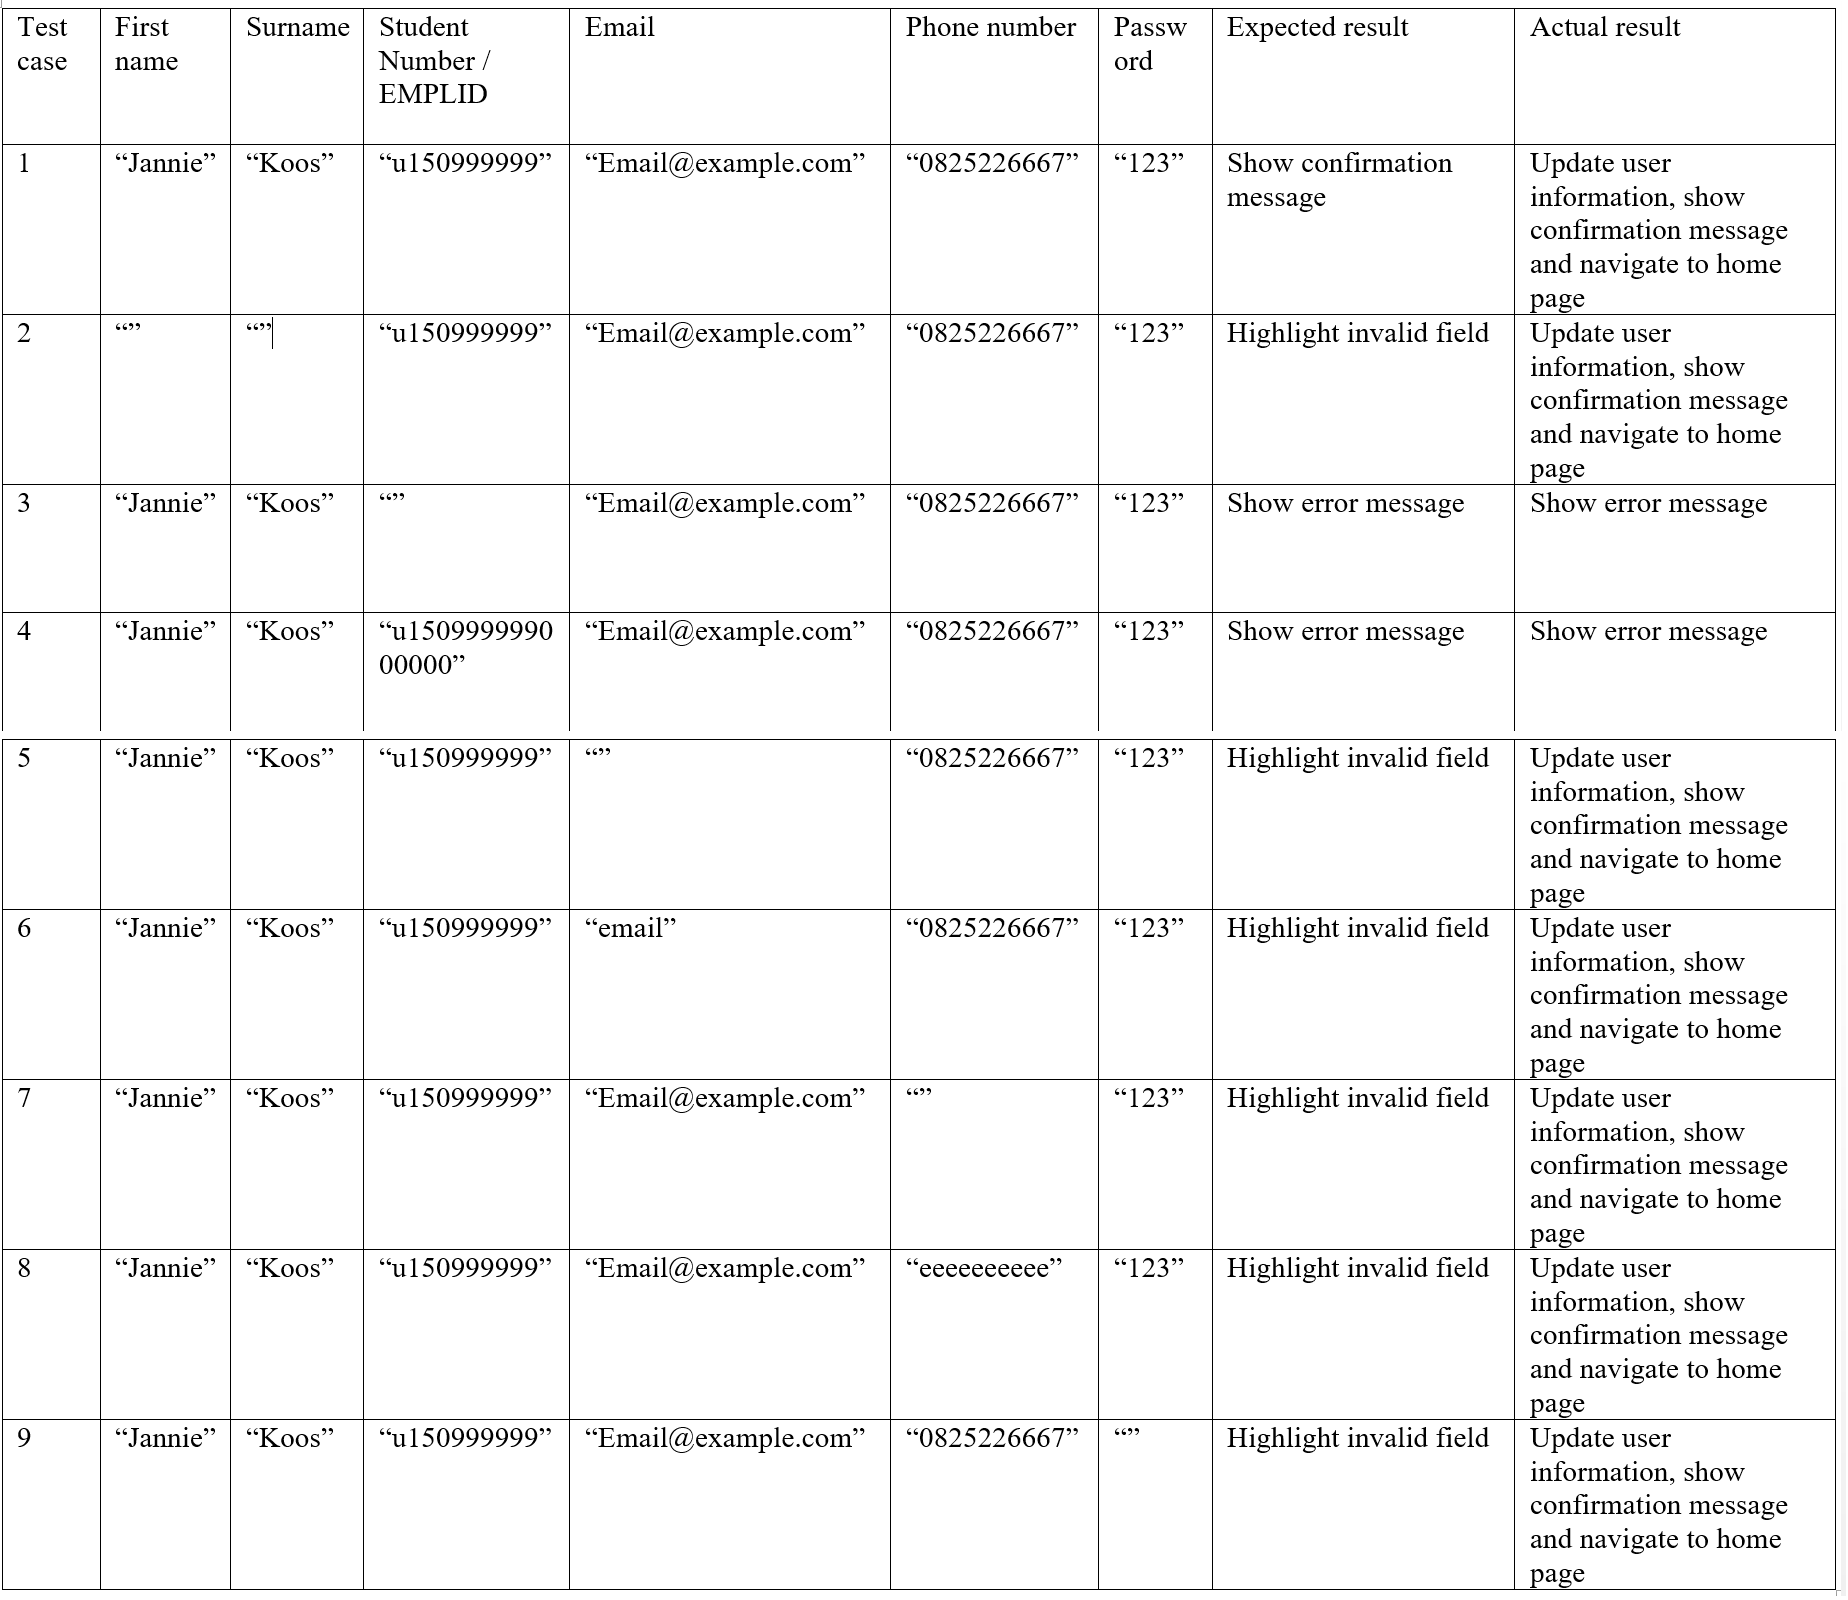
\includegraphics[width=180mm]{10.png}
\end{figure}

\begin{figure}[H]
\hspace*{-2.5cm} 
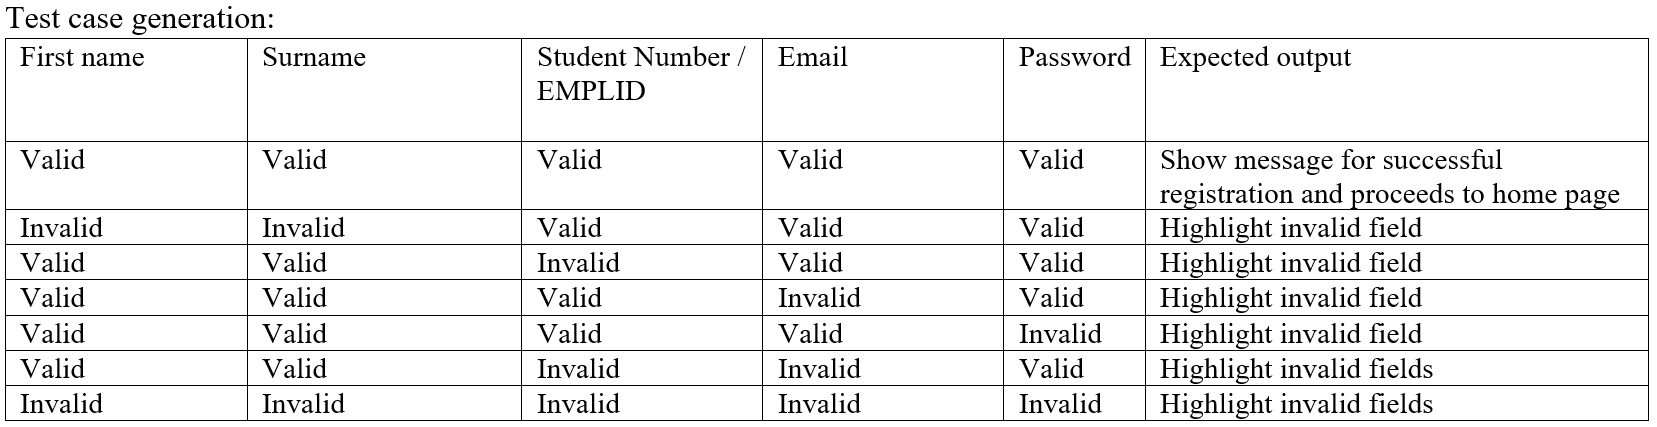
\includegraphics[width=180mm]{11.png}
\end{figure}

\subsection{Delete user profile}
\begin{figure}[ht!]
\hspace*{-2.5cm} 
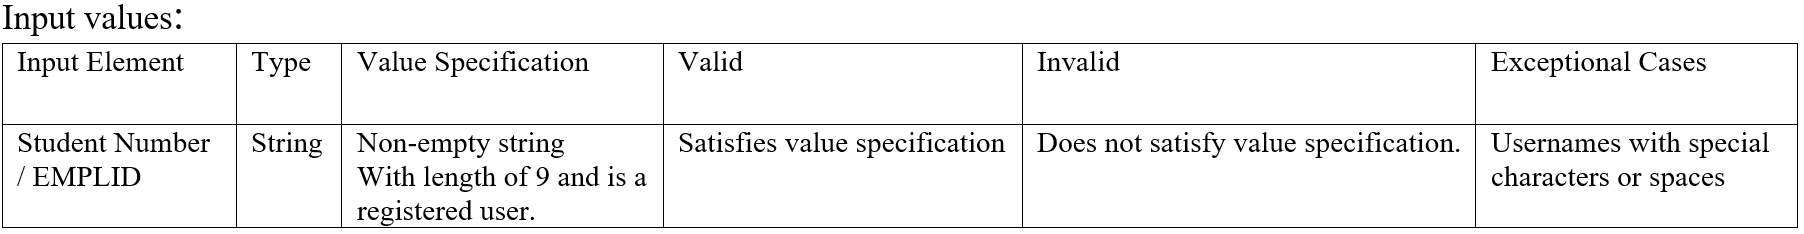
\includegraphics[width=180mm]{12.png}
\end{figure}

\subsection{Manage user information}
\begin{figure}[ht!]
\hspace*{-2.5cm} 
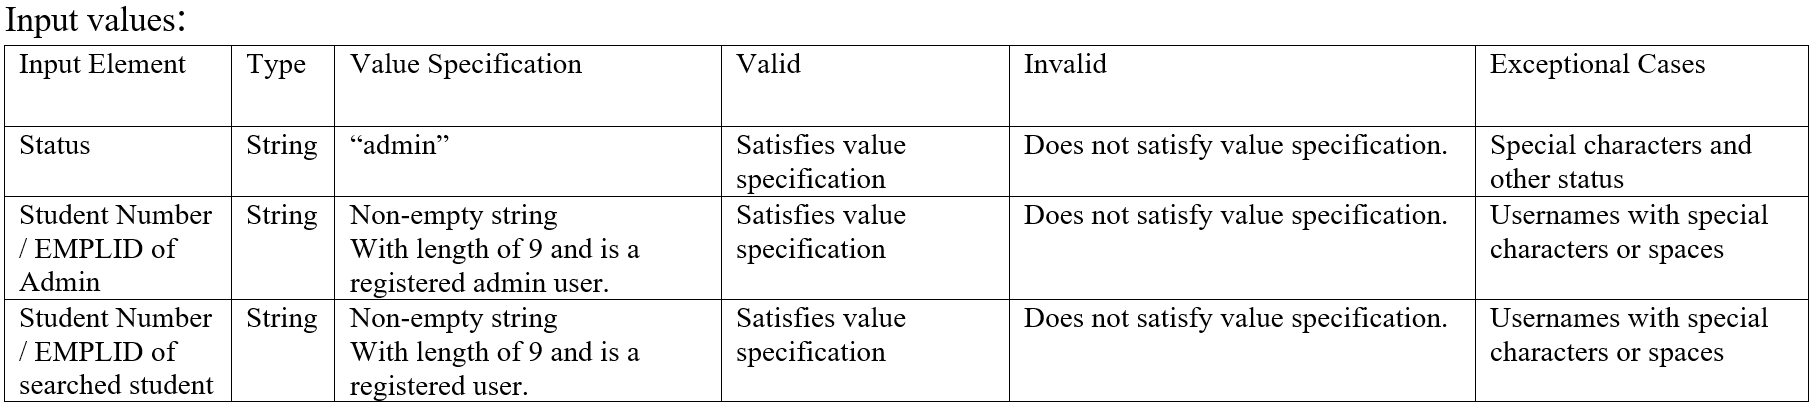
\includegraphics[width=180mm]{13.png}
\end{figure}

\begin{figure}[ht!]
\hspace*{-2.5cm} 
\includegraphics[width=180mm]{14_1.png}
\end{figure}

\clearpage

\section{Non-functional requirements}
1.	Security\\
2.	User interface\\
3.	Performance\\

\subsection{Security}
•	It is possible to change your user privileges to admin by changing the status of the user in the URL to “admin” at any page.\\
o	Once changing status to admin the users can officially give admin rights to themselves and other users.\\
•	Users can edit their user information to be empty strings especially for the password.\\
o	A password is not required to change the password or any other user information.\\
•	Users can login as other users by changing the user field in the URL to any valid user name.\\


\subsection{User interface}
•	Features are hidden based on user status i.e. manage users tab is hidden to guest users, but is visible to admin users\\

\subsection{Performance}
\begin{figure}[ht!]
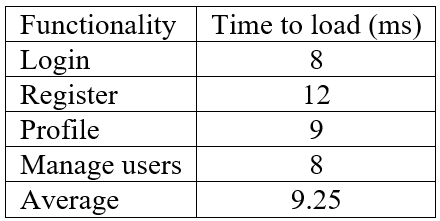
\includegraphics[width=60mm]{15.png}
\end{figure}
Performance-wise the pages were relatively fast and had nearly no noticeable loading time.
\end{document}
